\chapter{The Ising Magnet and the Liquid--Gas Transition}

We begin from a phenomenon everybody knows: boiling water, liquid turning into vapor, and a sharp change in density that we recognize as a phase transition. Leonard Susskind's point in this lecture is that we can understand that transition without following the standard van der Waals route. Instead we go back to a system already in our hands, the Ising magnet, and watch the same mathematics reappear in a different physical language. These notes follow that path closely, keeping the lecture's order and a few blackboard frames where the argument is visibly assembled on the board; the lecture record behind this chapter also reflects the curation work of LazyingArt LLC and Video2Book.

\section{From Boiling Water to the Ising Magnet}

The opening move is deliberately indirect. We are after the liquid--gas transition, but we are not going to attack it in the usual way. The claim is stronger and more interesting than a mere analogy: the Ising magnet provides a mathematically equivalent description of the same kind of transition.

That immediately explains why the lecture backs up before it goes forward. Before any talk about fluids, boxes, or chemical potential, we first rebuild the Ising model. We remind ourselves where the energy lives, what a broken bond costs, how an external field enters, and why mean field is good enough to reveal the qualitative mechanism of a phase transition. Only then do we reinterpret the same structure as a lattice gas.

\section{Recap of Ising Energetics and Mean Field}

At each lattice site \(i\) we place a spin
\begin{equation}
\sigma_i=\pm 1.
\end{equation}
In the Ising model the energy is not attached to a site by itself. It is attached to links between neighboring sites. With the sign convention used in this lecture, the energy is
\begin{equation}
E_{\text{Ising}}=-J\sum_{\langle ij\rangle}\sigma_i\sigma_j+h\sum_i \sigma_i.
\end{equation}
The first sum runs over nearest-neighbor links \(\langle ij\rangle\), not over sites. The constant \(J\) tells us how costly it is to break a bond.

For one link, the contribution is \(-J\sigma_i\sigma_j\). If the neighbors are parallel, \(\sigma_i\sigma_j=+1\), so the link energy is \(-J\). If they are anti-parallel, \(\sigma_i\sigma_j=-1\), so the link energy is \(+J\). Therefore the energy cost of breaking a bond is
\begin{equation}
\Delta E_{\text{broken bond}}=(+J)-(-J)=2J.
\end{equation}
This is one of the lecture's recurrent themes: it is the energy difference that matters, not the absolute zero of energy.

If all spins are aligned, the energy is as low as it can be. On an infinite hypercubic lattice in \(d\) dimensions, each site has \(2d\) neighbors, and because every link joins two sites, the total number of links is
\begin{equation}
N_{\text{links}}=d\,N_{\text{sites}}.
\end{equation}
Thus the completely aligned state has energy
\begin{equation}
E_{\text{ground}}=-J\,N_{\text{links}}=-J\,d\,N_{\text{sites}}.
\end{equation}
But this constant ground-state energy can be shifted away. Statistical mechanics only cares about differences between configurations.

The second term,
\begin{equation}
E_{\text{field}}=h\sum_i \sigma_i,
\end{equation}
acts on sites rather than links. In this convention, positive \(h\) lowers the energy when \(\sigma_i=-1\). So the two pieces of the Hamiltonian compete in a clear way: the link term wants neighboring spins to line up, while the field term favors one orientation over the other.

Now we recall the mean-field approximation. The lecture is very explicit about what it is good for and where it fails. In one dimension it gives the wrong qualitative answer: it predicts a phase transition where there is none. In two dimensions and higher it becomes useful, and by three dimensions, with six nearest neighbors, it is already quite good qualitatively. The reason is simple. The more neighbors a spin has, the more reasonable it becomes to replace the actual environment by an average one.

\begin{remark}
The sign of the field drifts verbally in the lecture, but the stable pair to keep is
\[
E_{\text{field}}=h\sum_i \sigma_i,
\qquad
\frac{yT}{2dJ}=\tanh(y-\beta h).
\]
With this convention, positive \(h\) favors \(\sigma=-1\). We keep that convention throughout.
\end{remark}

\section{Self-Consistency for the Average Spin}

The mean-field construction begins with one spin, drawn on the board and surrounded by its neighbors. We imagine it deep in the interior of a large sample, so that every site sees the same average environment.

\begin{figure}[t]
\centering

\includegraphics[width=0.82\textwidth]{lecture_10_figure_02.png}
\caption{Mean-field self-consistency for \(\bar{\sigma}\). The frame preserves both the neighbor sketch and the board equation, although the right edge is cropped.}
\end{figure}

\begin{figure}[t]
\centering
\begin{tikzpicture}[scale=1.15]
\fill (0,0) circle (2.4pt);
\node[below] at (0,-0.1) {$\sigma$};

\node at (1.6,0) {$\times$};
\node at (-1.6,0) {$\times$};
\node at (0,1.35) {$\times$};
\node at (0,-1.35) {$\times$};

\draw (0.18,0) -- (1.15,0);
\draw (-0.18,0) -- (-1.15,0);
\draw (0,0.18) -- (0,0.95);
\draw (0,-0.18) -- (0,-0.95);

\node[right] at (1.95,0.25) {$\bar{\sigma}$};
\node[left] at (-1.95,0.25) {$\bar{\sigma}$};
\node[above] at (0,1.62) {$\bar{\sigma}$};
\node[below] at (0,-1.62) {$\bar{\sigma}$};
\end{tikzpicture}
\caption{The mean-field picture: one spin interacting with \(2d\) neighbors, each replaced by the same average value \(\bar{\sigma}\).}
\end{figure}

Each of the \(2d\) neighbors is replaced by the average spin \(\bar{\sigma}\). The one-spin energy is therefore
\begin{equation}
E_{\text{mf}}(\sigma)=(-2dJ\,\bar{\sigma}+h)\sigma.
\end{equation}
This is exactly the coefficient structure visible on the board. The frame does not visibly show the factor of \(\beta\), because \(\beta\) enters only when we pass from the energy to the Boltzmann weight.

It is convenient to name the coefficient
\begin{equation}
A_{\text{mf}}=-2dJ\,\bar{\sigma}+h,
\qquad
E_{\text{mf}}(\sigma)=A_{\text{mf}}\sigma.
\end{equation}
Now we have reduced the many-spin problem to an ordinary one-spin statistical mechanics problem in the background of a parameter \(\bar{\sigma}\).

The one-spin partition function is
\begin{align}
Z_1
&=\sum_{\sigma=\pm1} e^{-\beta A_{\text{mf}}\sigma}
= e^{-\beta A_{\text{mf}}}+e^{\beta A_{\text{mf}}}
=2\cosh(\beta A_{\text{mf}}).
\end{align}
The thermal average of the chosen spin is
\begin{align}
\langle \sigma\rangle
&=\frac{\sum_{\sigma=\pm1}\sigma\,e^{-\beta A_{\text{mf}}\sigma}}
{\sum_{\sigma=\pm1}e^{-\beta A_{\text{mf}}\sigma}} \\
&=\frac{e^{-\beta A_{\text{mf}}}-e^{\beta A_{\text{mf}}}}
{e^{-\beta A_{\text{mf}}}+e^{\beta A_{\text{mf}}}}
=-\tanh(\beta A_{\text{mf}}) \\
&=\tanh\!\big[\beta(2dJ\,\bar{\sigma}-h)\big].
\end{align}

Now comes the self-consistency trick. The average spin of the chosen site is assumed to be the same as the average of its neighbors. In a large homogeneous sample, deep in the interior, that is exactly the mean-field assumption. Therefore
\begin{equation}
\bar{\sigma}=\tanh\!\big[\beta(2dJ\,\bar{\sigma}-h)\big].
\end{equation}
That is the mean-field equation determining \(\bar{\sigma}\).

The lecture then makes the standard simplifying substitution
\begin{equation}
y=2dJ\,\beta\,\bar{\sigma}.
\end{equation}
Since \(\beta=1/T\), this means
\begin{equation}
\bar{\sigma}=\frac{yT}{2dJ}.
\end{equation}
Substituting into the self-consistency condition gives the reduced equation
\begin{equation}
\frac{yT}{2dJ}=\tanh(y-\beta h).
\end{equation}
This is where the lecture wants to start over. Having compressed the many-spin system into one nonlinear equation, we are ready to solve it geometrically.

\section{Graphical Solution and the Critical Temperature}

The board is then cleared down to a single visible equation.

\begin{figure}[t]
\centering

\includegraphics[width=0.78\textwidth]{lecture_10_figure_03.png}
\caption{The reduced mean-field equation just before the graph is drawn. The visible equation is the stable form to keep.}
\end{figure}

The lecturer's next move is: forget the clutter, set the field to zero, and ask what the graph looks like. With \(h=0\), the reduced equation becomes
\begin{equation}
\frac{yT}{2dJ}=\tanh y.
\end{equation}
The left-hand side is a straight line through the origin. Its slope is \(T/(2dJ)\). The right-hand side is the fixed curve \(\tanh y\).

\begin{figure}[t]
\centering
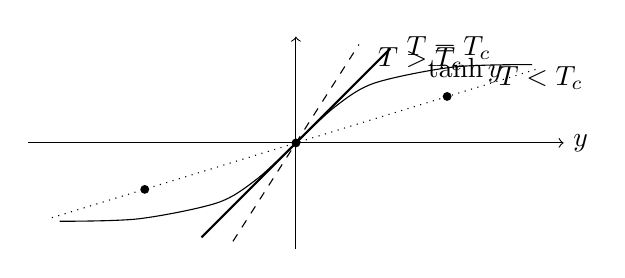
\begin{tikzpicture}[scale=1.0]
\draw[->] (-3.4,0) -- (3.4,0) node[right] {$y$};
\draw[->] (0,-1.35) -- (0,1.35);

\draw[smooth] plot coordinates {
(-3,-0.995) (-2,-0.964) (-1,-0.761) (-0.5,-0.462) (0,0)
(0.5,0.462) (1,0.761) (2,0.964) (3,0.995)};
\node at (2.15,0.92) {$\tanh y$};

\draw[dashed] (-0.8,-1.25) -- (0.8,1.25);
\node[right] at (0.92,1.06) {$T>T_c$};

\draw[thick] (-1.2,-1.2) -- (1.2,1.2);
\node[right] at (1.28,1.2) {$T=T_c$};

\draw[dotted] (-3.1,-0.95) -- (3.1,0.95);
\node[right] at (2.45,0.82) {$T<T_c$};

\fill (-1.92,-0.59) circle (1.6pt);
\fill (0,0) circle (1.6pt);
\fill (1.92,0.59) circle (1.6pt);
\end{tikzpicture}
\caption{Graphical solution of the mean-field equation at \(h=0\). At high temperature the only intersection is \(y=0\). At \(T_c\) the line is tangent at the origin. Below \(T_c\) two additional nonzero branches appear.}
\end{figure}

Now we read the graph exactly as the lecture reads it. At high temperature the line is steep, so the only intersection is the origin. Therefore
\begin{equation}
y=0,
\qquad
\bar{\sigma}=0.
\end{equation}
There is no magnetization.

Lower the temperature and the slope decreases. At a special temperature the line just hugs the curve at the origin. The slope of \(\tanh y\) at the origin is
\begin{equation}
\left.\frac{d}{dy}\tanh y\right|_{y=0}=1,
\end{equation}
so the tangency condition is
\begin{equation}
\frac{T_c}{2dJ}=1,
\end{equation}
and therefore
\begin{equation}
T_c=2dJ.
\end{equation}
This is the mean-field critical temperature.

If we lower the temperature still further, the line becomes shallower. Then two new intersections appear, one at positive \(y\) and one at negative \(y\). Strictly speaking the origin remains an intersection, but it is no longer the branch the system chooses. This is exactly the lecture's phrasing: the system does not go there. It chooses one of the nonzero solutions, so the magnetization becomes nonzero.

That is the phase transition in mean field. Above \(T_c\), thermal fluctuations win and the average magnetization is zero. Below \(T_c\), the tendency to line up wins and the system becomes spontaneously magnetized.

The lecture also makes an important accuracy remark here. The formula \(T_c=2dJ\) is not exact. It is a mean-field estimate. It becomes exact only when \(d\) is large. In two dimensions it is off by a noticeable amount; in three dimensions it is already fairly good. But it gets the qualitative story exactly right, and for this lecture that is the point.

For magnets one often calls \(T_c\) the Curie temperature. In the more general language of phase transitions it is simply the critical temperature.

\section{From Branch Selection to the \(T\)-\(h\) Plane}

At this point the lecture changes from equation solving to interpretation. Once the two symmetry-related nonzero solutions appear, the system ``doesn't quite know what to do.'' Should it choose the positive branch or the negative branch? The symmetry of the problem alone does not decide. If we flip every spin, we get the same problem back again.

The answer is that an arbitrarily small field removes the ambiguity. In practice the experimentalist controls two parameters: the temperature and the external field \(h\). The coupling \(J\) belongs to the material; if we want to change \(J\), we usually have to change the substance itself. So the natural plane to draw is the \(T\)-\(h\) plane.

Because we have fixed the convention \(E_{\text{field}}=h\sum_i \sigma_i\), a positive field favors \(\sigma=-1\), while a negative field favors \(\sigma=+1\). Equivalently, in the reduced equation the curve \(\tanh(y-\beta h)\) is shifted horizontally, and the sign of \(h\) selects one of the two nonzero branches.

\begin{figure}[t]
\centering
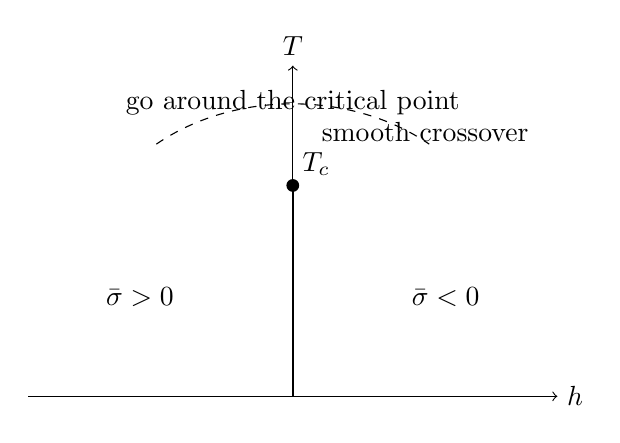
\begin{tikzpicture}[scale=1.05]
\draw[->] (-3.2,0) -- (3.2,0) node[right] {$h$};
\draw[->] (0,0) -- (0,4.0) node[above] {$T$};

\draw[thick] (0,0) -- (0,2.55);
\fill (0,2.55) circle (2.2pt);
\node[above right] at (0,2.55) {$T_c$};

\node at (-1.85,1.2) {$\bar{\sigma}>0$};
\node at (1.85,1.2) {$\bar{\sigma}<0$};
\node at (1.6,3.2) {smooth crossover};

\draw[dashed] (-1.65,3.05) .. controls (-0.7,3.7) and (0.7,3.7) .. (1.65,3.05);
\node at (0,3.55) {go around the critical point};
\end{tikzpicture}
\caption{The mean-field \(T\)-\(h\) plane. With the convention \(E_{\text{field}}=h\sum_i\sigma_i\), the positive-magnetization branch lies at \(h<0\) and the negative-magnetization branch at \(h>0\). Below \(T_c\), crossing \(h=0\) forces a jump from one branch to the other.}
\end{figure}

At high temperature and zero field, the magnetization is zero. At zero temperature, by contrast, the system is fully lined up, so \(\bar{\sigma}=\pm1\). Between these limits the phase diagram organizes the whole story.

\subsection{Question \& Answer}

\paragraph{Question.} What jumps, and what does not?

\paragraph{Answer.} The crucial distinction is between approaching the critical point and crossing the coexistence line. As \((T,h)\to(T_c,0)\) from any direction, the magnetization tends to zero:
\begin{equation}
\lim_{(T,h)\to(T_c,0)} \bar{\sigma}(T,h)=0.
\end{equation}
So the critical point itself is continuous.

But if we keep \(T<T_c\) fixed and vary the field through \(h=0\), then the magnetization jumps from one nonzero branch to the other:
\begin{equation}
\bar{\sigma}(T,0^\pm)=\pm m_0(T),
\qquad
m_0(T)>0,
\qquad
T<T_c.
\end{equation}
The sign convention tells us which side of the axis corresponds to which branch, but the important fact is the discontinuity itself.

\paragraph{Question.} What happens exactly on the line \(h=0\) below \(T_c\)?

\paragraph{Answer.} In the idealized perfectly symmetric problem, the system cannot decide. The two branches are equally available. In a real experiment one never turns off every bias completely, so some tiny residual field or imperfection picks one branch. That is why the lecture says the system ``doesn't know what to do'' exactly on the axis.

\paragraph{Question.} Can one move from negative magnetization to positive magnetization without a jump?

\paragraph{Answer.} Yes, provided one is allowed to move in the full \((T,h)\) plane instead of keeping \(T\) fixed. If we go around the critical point, passing through the high-temperature region, the magnetization changes smoothly from one sign to the other. So both statements are true. At fixed \(T<T_c\) there is a jump across \(h=0\); globally there is still a continuous path around the critical point.

The lecture briefly alludes to the taxonomy of phase transitions, but does not pursue it. The geometric statement above is the one that matters here.

\section{Chemical Potential and the Box Picture}

At this stage the lecturer says, in effect: now we know enough about magnets, but I am interested in the liquid--gas transition. So the lecture pivots to a permeable box.

Imagine a region of space whose interior is at lower potential energy than the exterior. The walls are permeable, so particles can come in and out. The energy difference between being inside and being outside is the chemical potential \(\mu\), understood here as the energy cost of removing a particle from the box.

\begin{figure}[t]
\centering
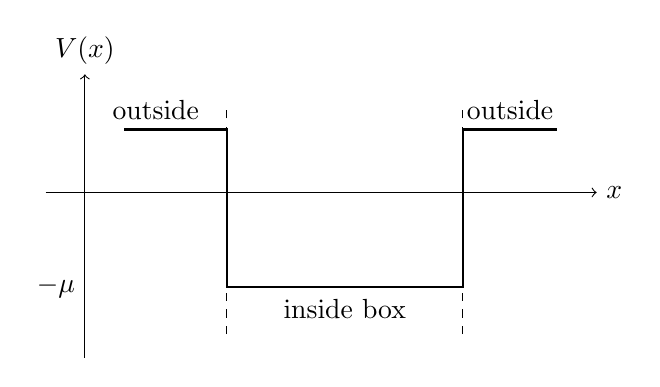
\begin{tikzpicture}[scale=1.0]
\draw[->] (-0.5,0) -- (6.5,0) node[right] {$x$};
\draw[->] (0,-2.1) -- (0,1.5) node[above] {$V(x)$};

\draw[thick] (0.5,0.8) -- (1.8,0.8) -- (1.8,-1.2) -- (4.8,-1.2) -- (4.8,0.8) -- (6.0,0.8);
\draw[dashed] (1.8,-1.8) -- (1.8,1.1);
\draw[dashed] (4.8,-1.8) -- (4.8,1.1);

\node at (0.9,1.05) {outside};
\node at (5.4,1.05) {outside};
\node at (3.3,-1.48) {inside box};
\node[left] at (0,-1.2) {$-\mu$};
\end{tikzpicture}
\caption{The permeable-box picture. Inside the box the one-particle energy is lower, so the equilibrium density depends on the chemical potential \(\mu\).}
\end{figure}

The Boltzmann factor always favors lower energy. So if the inside of the box is lower in energy, the density inside rises. The stronger the chemical potential, the more the box wants to pull particles in. The lecture does not use this picture to discuss chemistry in any detail. It uses it to isolate a variable that controls density.

Because particles can cross the walls, the number of particles is itself part of the configuration. If we were to set up the statistical mechanics in full, we would use the grand-canonical partition function
\begin{equation}
Z=\sum_N \sum_{\text{conf}_N} e^{-\beta E+\beta\mu N}.
\end{equation}
Here the sum is not only over positions and momenta, but also over the particle number \(N\). The lecture does not carry out the calculation. It only needs the meaning of the formula: \(\mu\) is the thing we adjust if we want to adjust the average density.

Now we can say what the liquid--gas transition looks like in this language. Hold the temperature fixed and vary the chemical potential. Then the density inside the box is some function of \(\mu\). In the gas phase the density is low. In the liquid phase the density is high. A liquid--gas transition is the place where, as we vary \(\mu\), that density changes discontinuously.

\begin{remark}
The lecture carefully avoids a pressure computation. One could in principle rewrite the discussion in terms of pressure, but that would require more thermodynamics than is done here. We keep the discussion at the level used in the lecture.
\end{remark}

\subsection{Question \& Answer}

\paragraph{Question.} How does one actually vary the chemical potential in practice?

\paragraph{Answer.} In the lecture the cleanest thought experiment is to lower the one-particle energy inside the box and thereby ``pull'' particles in. But the lecturer immediately admits that this is not how one usually does it for an ordinary fluid. In practice the most accessible control is pressure. Pressure changes the density, and the boiling point depends on it. So the box picture with \(\mu\) is the conceptual model, while pressure is the usual laboratory handle.

\paragraph{Question.} What becomes of the jump if we go above the critical point?

\paragraph{Answer.} Then the jump disappears. Above the critical temperature the density changes smoothly as we vary the control parameter. The sharp distinction between gas and liquid survives only below the critical point. And, just as in the magnetic case, one can go from low density to high density without a jump by going around the critical point through the high-temperature region.

\section{The Lattice Gas Hidden Inside the Ising Model}

Now comes the lecture's main translation. What does the Ising magnet have to do with a fluid? Before giving the dictionary, the lecture states the two ingredients needed for a liquid--gas transition.

First, there must be hard-core repulsion: two molecules cannot sit on top of one another. Second, there must be a little attraction when they are near but not coincident. The standard molecular picture has exactly this form: very strong short-distance repulsion, plus a modest short-range attraction.

The striking claim is that the Ising model supplies both ingredients automatically.

We reinterpret the all-down state as empty space. Then we say:
\begin{equation}
\sigma_i=-1 \Longleftrightarrow n_i=0,
\qquad
\sigma_i=+1 \Longleftrightarrow n_i=1.
\end{equation}
So \(\sigma=-1\) means no particle on the site, and \(\sigma=+1\) means one particle on the site.

\begin{figure}[t]
\centering

\includegraphics[width=0.74\textwidth]{lecture_10_figure_04.png}
\caption{The moment where the board explicitly identifies \(\sigma=-1\) with an empty lattice site.}
\end{figure}

\begin{figure}[t]
\centering
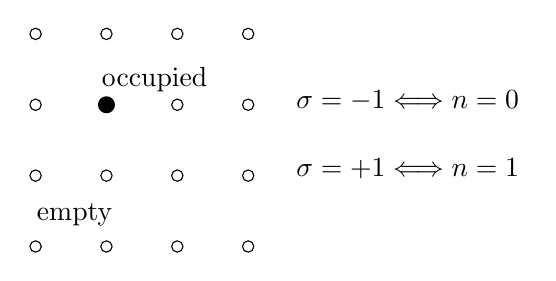
\begin{tikzpicture}[scale=0.9]
\foreach \x in {0,1,2,3}
  \foreach \y in {0,1,2,3}
    \draw (\x,\y) circle (0.08);

\fill (1,2) circle (0.12);

\node at (5.25,2.05) {$\sigma=-1 \Longleftrightarrow n=0$};
\node at (5.25,1.1) {$\sigma=+1 \Longleftrightarrow n=1$};
\node at (1.68,2.36) {occupied};
\node at (0.55,0.45) {empty};
\end{tikzpicture}
\caption{The lattice-gas dictionary. Since \(\sigma\) can only be \(\pm1\), the model automatically forbids double occupancy.}
\end{figure}

Immediately we get the hard core. The Ising variable does not allow \(\sigma=2\). So it does not allow two particles on the same site. Occupation is either \(0\) or \(1\), never more. The infinite short-distance repulsion is built in from the start.

The next question is whether these particles attract. For that we simply count broken bonds. We subtract the constant ground-state energy and declare the empty lattice to have zero energy.

\begin{figure}[t]
\centering

\includegraphics[width=0.78\textwidth]{lecture_10_figure_05.png}
\caption{The bookkeeping step where the Ising energy is re-read as particle energetics: one particle, two separated particles, and two nearby particles.}
\end{figure}

Let us do the counting in two dimensions, exactly as in the lecture. One particle means one spin flipped up in an otherwise down background. That breaks four bonds. Since each broken bond costs \(2J\),
\begin{equation}
E_{1\text{ particle}}=4(2J)=8J.
\end{equation}
Two well-separated particles simply double that cost:
\begin{equation}
E_{2\text{ particles, far apart}}=16J.
\end{equation}
But if the two particles are nearest neighbors, the bond between them is not broken, because both spins are up. Then only six bonds are broken, so
\begin{equation}
E_{2\text{ particles, nearest neighbors}}=6(2J)=12J.
\end{equation}
Therefore bringing two particles from far separation to one lattice spacing lowers the energy by
\begin{equation}
\Delta E_{\text{nn attraction}}=12J-16J=-4J.
\end{equation}
That is the short-range attraction.

\begin{figure}[t]
\centering
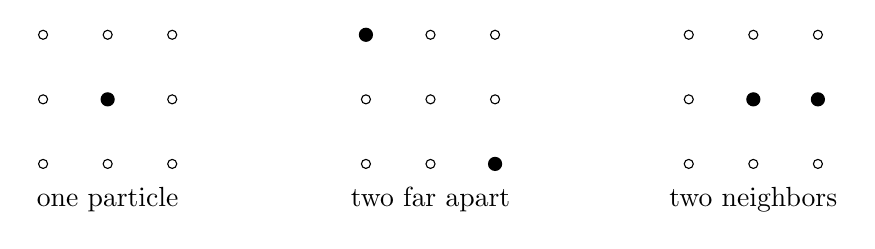
\begin{tikzpicture}[scale=0.82]
\foreach \x in {0,1,2}
  \foreach \y in {0,1,2}
    \draw (\x,\y) circle (0.07);
\fill (1,1) circle (0.11);
\node at (1,-0.55) {one particle};

\begin{scope}[xshift=5.0cm]
\foreach \x in {0,1,2}
  \foreach \y in {0,1,2}
    \draw (\x,\y) circle (0.07);
\fill (0,2) circle (0.11);
\fill (2,0) circle (0.11);
\node at (1,-0.55) {two far apart};
\end{scope}

\begin{scope}[xshift=10.0cm]
\foreach \x in {0,1,2}
  \foreach \y in {0,1,2}
    \draw (\x,\y) circle (0.07);
\fill (1,1) circle (0.11);
\fill (2,1) circle (0.11);
\node at (1,-0.55) {two neighbors};
\end{scope}
\end{tikzpicture}
\caption{The three lattice configurations whose bond counting gives \(8J\), \(16J\), and \(12J\) in two dimensions.}
\end{figure}

So the Ising system, read as a lattice gas, has exactly the two features the lecture asked for: infinite hard-core repulsion at zero separation, and modest attraction at one lattice spacing.

Now let us restore the field term. If a site changes from empty to occupied, then \(\sigma\) changes from \(-1\) to \(+1\), so the field contribution changes by
\begin{equation}
\Delta E_h = 2h.
\end{equation}
Thus an isolated particle in two dimensions has energy
\begin{equation}
E_{1\text{ particle}}=8J+2h
\end{equation}
in this counting convention. The point is not the exact offset, which the lecture treats as conventional. The point is that \(J\) controls the interaction between neighboring particles, while \(h\) changes the one-body cost of having a particle present. That is exactly how a tunable chemical potential should behave.

\begin{remark}
The identification of \(h\) with the thermodynamic chemical potential is only clean up to sign convention and an additive constant. The lecture's stable statement is the structural one: \(h\) tunes the one-particle energy without changing the interaction strength \(J\).
\end{remark}

Finally, we need the density. The occupation variable is
\begin{equation}
n_i=\frac{1+\sigma_i}{2},
\end{equation}
because this gives \(n_i=0\) when \(\sigma_i=-1\) and \(n_i=1\) when \(\sigma_i=+1\). Averaging gives
\begin{equation}
\rho=\langle n_i\rangle=\frac{1+\bar{\sigma}}{2}
=\frac12+\frac{\bar{\sigma}}{2}.
\end{equation}
This is another important beat in the lecture: the density is not \(\bar{\sigma}\), but a shifted version of it, because \(\sigma=-1\) means zero particles, not minus one particle.

Now the magnetic phase diagram translates directly into the fluid one. Above the critical temperature, varying \(h\) changes \(\bar{\sigma}\) smoothly, so varying the chemical potential changes the density smoothly. Nothing dramatic happens. Below the critical temperature, by contrast, \(\bar{\sigma}\) jumps across the coexistence line, and therefore the density jumps as well:
\begin{equation}
\Delta \rho = \frac12 \Delta \bar{\sigma}.
\end{equation}
Negative \(\bar{\sigma}\) means low density, positive \(\bar{\sigma}\) means high density. So the magnetic jump becomes the jump from vapor to liquid. In that sense boiling is just the lattice-gas translation of spontaneous magnetization.

This is the lecture's main conclusion: the magnet and the fluid are not merely similar. They are the same mathematical system wearing different physical interpretations.

The lecture closes the statistical mechanics portion with one final remark. Near the critical point there are many interesting singular behaviors, described by critical exponents. Those exponents depend far less on microscopic details than one might have expected. In particular, the magnetic transition and the liquid--gas transition belong to the same critical-behavior class. That is the universality statement the lecture wants us to carry away.

\section{Summary}

We began with boiling water and took the long way around. First we rebuilt the Ising model: spins on a lattice, energy stored on links, a broken-bond cost of \(2J\), and a field term that acts on individual sites. Then mean field reduced the many-spin system to one spin in an averaged neighborhood, leading to the self-consistency equation
\[
\bar{\sigma}=\tanh\!\big[\beta(2dJ\bar{\sigma}-h)\big]
\]
and the reduced form
\[
\frac{yT}{2dJ}=\tanh(y-\beta h).
\]
From the graph of a line against \(\tanh y\), we read off the mean-field critical temperature \(T_c=2dJ\), the emergence of symmetry-broken branches below \(T_c\), and the distinction between continuity at the critical point and the jump across the coexistence line.

Then the same mathematics was read as a lattice gas. Empty and occupied sites became \(\sigma=-1\) and \(\sigma=+1\). Hard-core exclusion was automatic. Explicit bond counting gave
\[
8J,\qquad 16J,\qquad 12J,
\]
showing a nearest-neighbor attraction of strength \(4J\). The field term supplied a tunable one-body cost, and the density became
\[
\rho=\frac{1+\bar{\sigma}}{2}.
\]
So the magnetization jump became a density jump, the magnetic phase diagram became the liquid--gas phase diagram, and the critical point of the magnet became the critical point of boiling.